\documentclass{article}
\usepackage[margin=1in]{geometry}
\usepackage{amsmath,amsthm,amssymb}
\usepackage{bbm,enumerate,mathtools}
\usepackage{tikz,pgfplots}
\usepackage{chessboard}
\usepackage[hidelinks]{hyperref}
\usepackage{multicol} % Problem 35
\usepackage{xstring} % Difficulty command
\usetikzlibrary{shapes.geometric}

\newenvironment{question}{\begin{trivlist}\item[\textbf{Question.}]}{\end{trivlist}}
\newenvironment{note}{\begin{trivlist}\item[\textbf{Note.}]}{\end{trivlist}}
\newenvironment{references}{\begin{trivlist}\item[\textbf{References.}]}{\end{trivlist}}
\newenvironment{related}{\begin{trivlist}\item[\textbf{Related.}]\end{trivlist}\begin{enumerate}}{\end{enumerate}}

\newcommand\score[1]{
\pgfmathsetmacro\pgfxa{#1+1}
\tikzstyle{scorestars}=[
  star,
  star points=5,
  star point ratio=2.25,
  draw,
  inner sep=3pt,
  anchor=outer point 5
]
  \begin{tikzpicture}[baseline]
    \draw[opacity=0] (0,-0.5) rectangle (0,0.2); % Workaround for whitespace at the bottom.
    \foreach \i in {1,...,4} {
      \pgfmathparse{(\i<=#1?"yellow":"gray")}
      \edef\starcolor{\pgfmathresult}
      \draw (\i*4.5ex,0) node[name=star\i,scorestars,fill=\starcolor]  {};
    }
  \end{tikzpicture}
}

\newcommand{\difficulty}[1]{%
  \IfEqCase{#1}{%
      {1}{
        
\begin{tikzpicture}[scale=0.7, baseline=0.9mm]%
          \definecolor{slopegreen}{rgb}{0.0, 0.5, 0.0}%
          \fill[slopegreen] (0.5,0.5) circle (0.5);%
        \end{tikzpicture}%
      }%
      {2}{
        
\begin{tikzpicture}[scale=0.7, baseline=0.9mm]%
          \definecolor{slopeblue}{rgb}{0.0, 0.44, 1.00}
          \fill[slopeblue] (0,0) rectangle (1,1);%
        \end{tikzpicture}%
      }%
      {3}{
\begin{tikzpicture}[scale=0.7, baseline=0.9mm]\fill (0,0.5)--(0.5, 0)--(1,0.5)--(0.5,1)--cycle; \end{tikzpicture}}%
      {4}{
\begin{tikzpicture}[scale=0.7, baseline=0.9mm]\fill (0.25,0)--(0,0.5)--(0.25,1)--(0.5,0.5)--cycle; \fill (0.75,0)--(0.5,0.5)--(0.75,1)--(1,0.5)--cycle;\end{tikzpicture}}%
      % you can add more cases here as desired
  }[\PackageError{difficulty}{Undefined difficulty level: #1}{}]%
}%
\newcommand{\rating}[2]{\difficulty{#1}\\\score{#2}\\}


\begin{document}
  Consider all configurations of nonattacking rooks on an $n\times n$ board up
  to dihedral action.

\begin{figure}[!h]
  \centering
  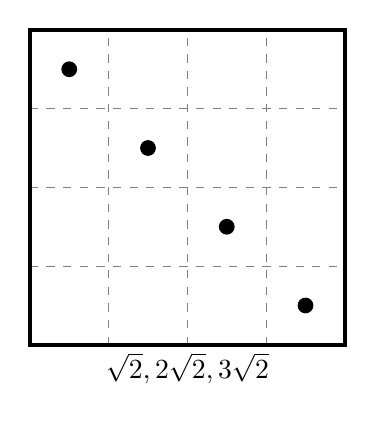
\begin{tikzpicture}
    % 1
    \draw[gray, dashed] (0,0) grid (4,4);
    \draw[ultra thick] (0,0) rectangle (4,4);
    \foreach \x/\y in {1/4,2/3,3/2,4/1} {
      \fill (\x - 0.5, \y - 0.5) circle (0.1cm);
    }
    \node at (2, -0.3) {$\sqrt{2}, 2\sqrt{2}, 3\sqrt{2}$};
  \end{tikzpicture}\hspace{1cm}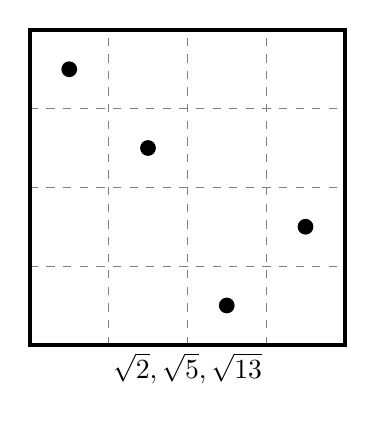
\begin{tikzpicture}
    % 2
    \draw[gray, dashed] (0,0) grid (4,4);
    \draw[ultra thick] (0,0) rectangle (4,4);
    \foreach \x/\y in {1/4,2/3,3/1,4/2} {
      \fill (\x - 0.5, \y - 0.5) circle (0.1cm);
    }
    \node at (2, -0.3) {$\sqrt{2}, \sqrt{5}, \sqrt{13}$};
  \end{tikzpicture}\hspace{1cm}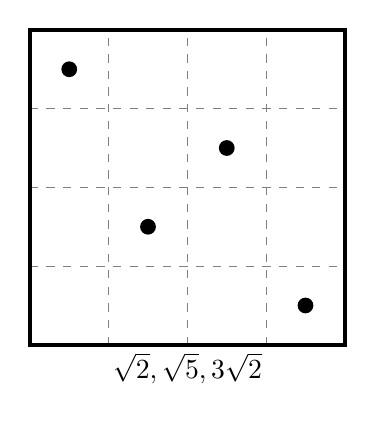
\begin{tikzpicture}
    % 3
    \draw[gray, dashed] (0,0) grid (4,4);
    \draw[ultra thick] (0,0) rectangle (4,4);
    \foreach \x/\y in {1/4,2/2,3/3,4/1} {
      \fill (\x - 0.5, \y - 0.5) circle (0.1cm);
    }
    \node at (2, -0.3) {$\sqrt{2}, \sqrt{5}, 3\sqrt{2}$};
  \end{tikzpicture}\vspace{3mm}\\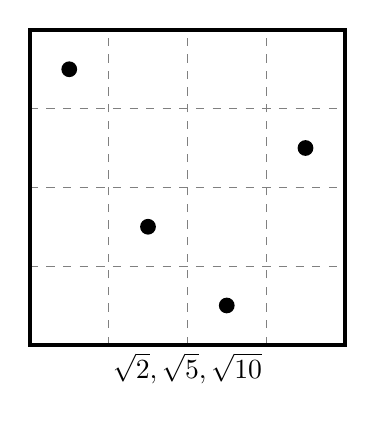
\begin{tikzpicture}
    % 4
    \draw[gray, dashed] (0,0) grid (4,4);
    \draw[ultra thick] (0,0) rectangle (4,4);
    \foreach \x/\y in {1/4,2/2,3/1,4/3} {
      \fill (\x - 0.5, \y - 0.5) circle (0.1cm);
    }
    \node at (2, -0.3) {$\sqrt{2}, \sqrt{5}, \sqrt{10}$};
  \end{tikzpicture}\hspace{1cm}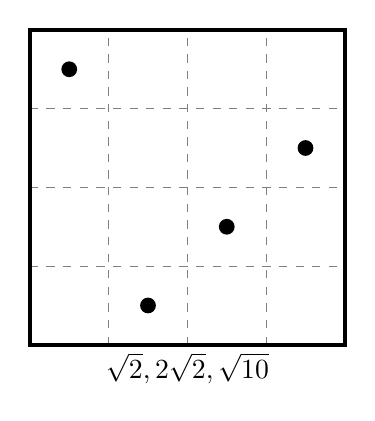
\begin{tikzpicture}
    % 5
    \draw[gray, dashed] (0,0) grid (4,4);
    \draw[ultra thick] (0,0) rectangle (4,4);
    \foreach \x/\y in {1/4,2/1,3/2,4/3} {
      \fill (\x - 0.5, \y - 0.5) circle (0.1cm);
    }
    \node at (2, -0.3) {$\sqrt{2}, 2\sqrt{2}, \sqrt{10}$};
  \end{tikzpicture}\hspace{1cm}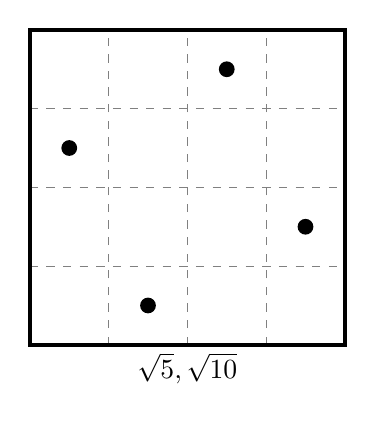
\begin{tikzpicture}
    % 6
    \draw[gray, dashed] (0,0) grid (4,4);
    \draw[ultra thick] (0,0) rectangle (4,4);
    \foreach \x/\y in {1/3,2/1,3/4,4/2} {
      \fill (\x - 0.5, \y - 0.5) circle (0.1cm);
    }
    \node at (2, -0.3) {$\sqrt{5}, \sqrt{10}$};
  \end{tikzpicture}\vspace{3mm}\\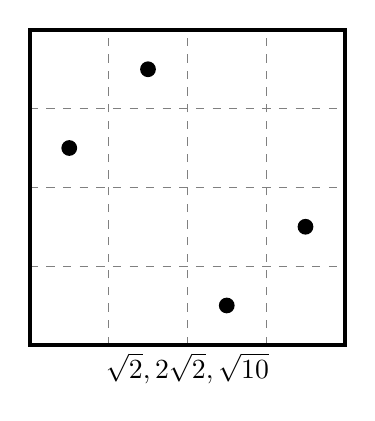
\begin{tikzpicture}
    % 7
    \draw[gray, dashed] (0,0) grid (4,4);
    \draw[ultra thick] (0,0) rectangle (4,4);
    \foreach \x/\y in {1/3,2/4,3/1,4/2} {
      \fill (\x - 0.5, \y - 0.5) circle (0.1cm);
    }
    \node at (2, -0.3) {$\sqrt{2}, 2\sqrt{2}, \sqrt{10}$};
  \end{tikzpicture}
  \caption{
    Each figure is marked with the distinct distances between pieces.
  }
\end{figure}

\begin{question}
  What is the minimum number of distinct distances on such a figure?
\end{question}
\begin{related}
  \item What if rooks are allowed to be in attacking positions?
  \item How many configurations of nonattacking rooks on the torus?
  \item Are any configurations of nonattacking rooks on the torus that can
    be meaningfully called a ``generalized Costas array''?
\end{related}
\begin{references}
  \item \url{https://en.wikipedia.org/wiki/Costas_array}
\end{references}
\end{document}
